\documentclass[a4paper, 11pt, report]{article}

\usepackage[slovak]{babel}
\usepackage[utf8]{inputenc}
\usepackage[T1]{fontenc}
\usepackage{times}
\usepackage{graphicx}
\usepackage{pdflscape}

\usepackage{geometry}
\geometry{text={170mm, 240mm}, left=20mm, top=30mm}

\setlength{\parindent}{4em}

\begin{document}

    \begin{titlepage}
        \begin{center}
            
\includegraphics[width=0.77 \linewidth]{FIT_logo.pdf} \\
            
            \vspace{\stretch{0.382}}
            {\Huge \textbf{Databázové systémy\,--\,Projekt 1.časť} \\[0.3em]
            \huge Dátový model (ERD), model prípadov užitia} \\[0.4em]
            {\LARGE 26. Banka}\\
            \vspace{\stretch{0.618}}
        \end{center}
        
        {\Large \today \hfill 
            \begin{tabular}{l l}
    				Patrik Sehnoutek & (xsehno01) \\
    				Dalibor Králik & (xkrali20) \\
    			\end{tabular}
		}
    \end{titlepage}
    
    
    \section{Zadanie}

    Navrhnite modul informačného systému banky pre správu účtov. Banka poskytuje dva druhy účtom, sporiaci a bežný účet. O sporiacom účte bude v systéme informácia o úroku a o bežnom účte bude informácia o poplatku za vedenie účtu. O učte nesmú chýbať informácie ako číslo účtu, dátum založenia, zostatok a IBAN. Modul musí evidovať klientov, ich účty a operácie s nimi. Predpokladajte, že každý účet má jedného vlastníka, ale s účtom môže disponovať viacero osôb, ktoré určí vlastník. Disponent ma zadaný limit, s ktorým môže disponovať. Operácie zahrnujú vklad na účet, výber z účtu a prevod na iný účet (rovnakej alebo inej banky) sú realizované pomocou bankového príkazu, o ktorom banka udržuje dáta, napríklad poradové číslo, dátum, čiastka a typ príkazu. Systém musí ukladať informácie o všetkých operáciách s účtom (kto zadal, kedy, aká operácia a čiastka, kto vykonal). So systémom vždy priamo komunikuje iba zamestnanec banky, ktorý môže vytvárať účty, rušiť účty, vytvárať nových klientov v systéme a rušiť klientov v systéme. O zamestnancovi bude v systéme evidované jeho základné informácie ako meno, priezvisko, bydlisko, kontaktné údaje a dátum narodenia. Systém musí tiež okrem iného poskytovať výpis z účtu, ktorý sa posiela vlastníkovi, tj. výpis všetkých operácií s účtom za dané obdobie.
    
    
    \newpage
    
    
    \section{Diagram prípadov užitia (Use Case Diagram)}
   
    Model prípadov užitia pozostáva z dvoch užívateľov klienta a zamestnanca. Zamestnanec ako privilegovaný užívateľ má na starosti administratívu účtov klientov, čo v sebe zahŕňa vytváranie, rušenie a správu účtov. Taktiež je jeho úlohou zakladanie a rušenie účtov samotných klientov. Druhým užívateľom je klient, ktorý má právo určiť disponentov svojho účtu, vytvárať bankové príkazy a manipulovať so zostatkom na účte: vklad a výber financií.
    
    \bigskip
    \begin{figure}[ht]
        \centering
        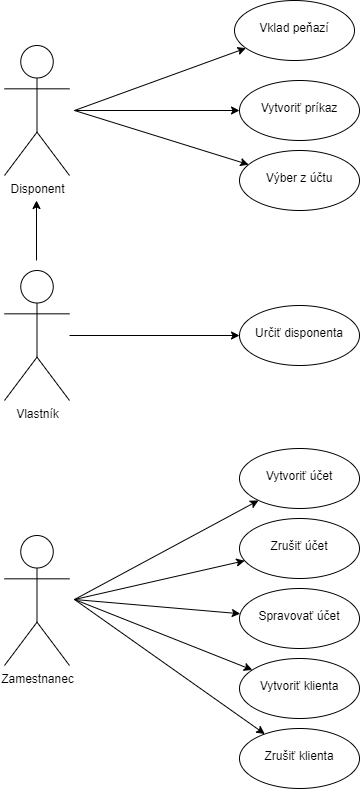
\includegraphics[width=0.50 \linewidth]{UseCase.png}\\
        \caption{Diagram prípadov užitia (Use Case Diagram)}
    \end{figure}
    
    \newpage
    
    
    \section{Dátový model (ERD)}
    
    Navrhnutý ER diagram obsahuje niekoľko silných a slabých entít. Entita \textbf{KLIENT} vlastní \textbf{ÚČET} a disponuje na ňom určitým limitom. Vlastníkom účtu môže byť iba jeden klient, ale disponovať ním môže niekoľko ďalších klientov, ktorých určí vlastník. Disponovanie s účtom v sebe zahŕňa tvorbu platobných \textbf{PRÍKAZOV} a možnosť \textbf{VÝPISU}, aby mal klient prehľad o zostatku a pohybe peňazí na účte. Tieto dve spomínané entity nemôžu existovať bez toho, aby mal užívateľ založený účet. Účet sa rozdeľuje na dva typy, \textbf{SPORIACI} a \textbf{BEŽNÝ}. Za bežný účet je vedený poplatok a sporiaci účet zahŕňa určitý úrok. Účet je spravovaný povereným \textbf{ZAMESTNANCOM} banky, ktorý môže mať na starosti niekoľko účtov.
    
    \bigskip
    %\begin{landscape}
		\begin{figure}[h]
			\centering
			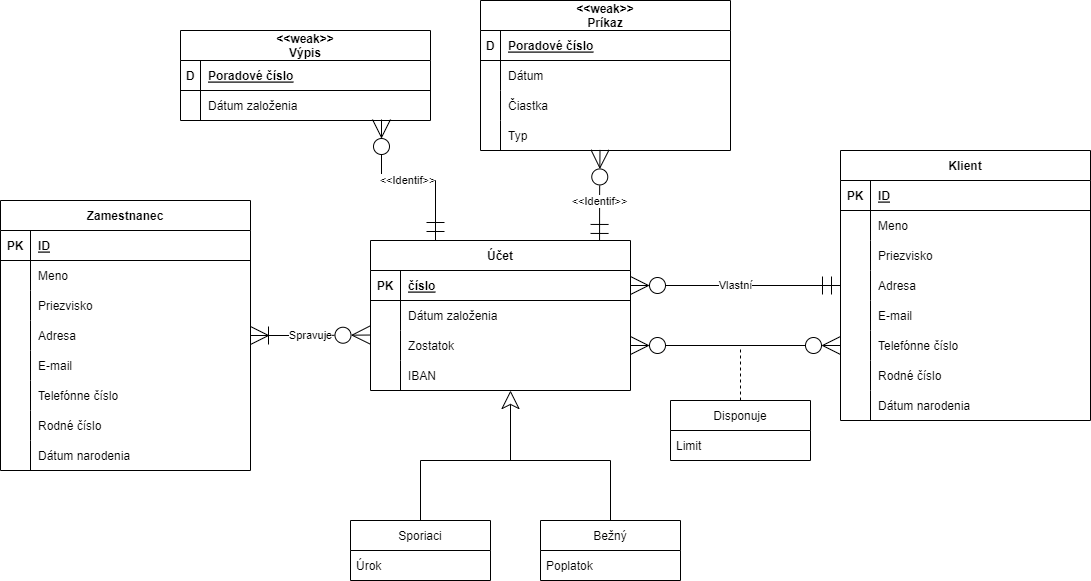
\includegraphics[width=0.95 \linewidth]{ERDiagram.png}
			\caption{Dátový model (ERD)}
		\end{figure}
	%\end{landscape}


\end{document}
